\section{Einphasiger Wechselrichter}

Ein einphasiger Wechselrichter wandelt eine konstante Gleichspannung $U_{DC}$ in eine
\textbf{wechselnde Ausgangsspannung} $u_2(t)$ mit vorgegebener Frequenz und Amplitude.

Typische Anwendungen:
\begin{itemize}
\item USV-Anlagen,
\item Photovoltaik-Wechselrichter,
\item Einphasenantriebe,
\item Netzgekoppelte Einspeiser.
\end{itemize}

Die Grundtopologie ist die \textbf{H-Brücke} mit vier steuerbaren Schaltern.

\subsection{Grundprinzip der H-Brücke}

% --- bestehende Grafik: H-Brücke ---
\begin{center}
    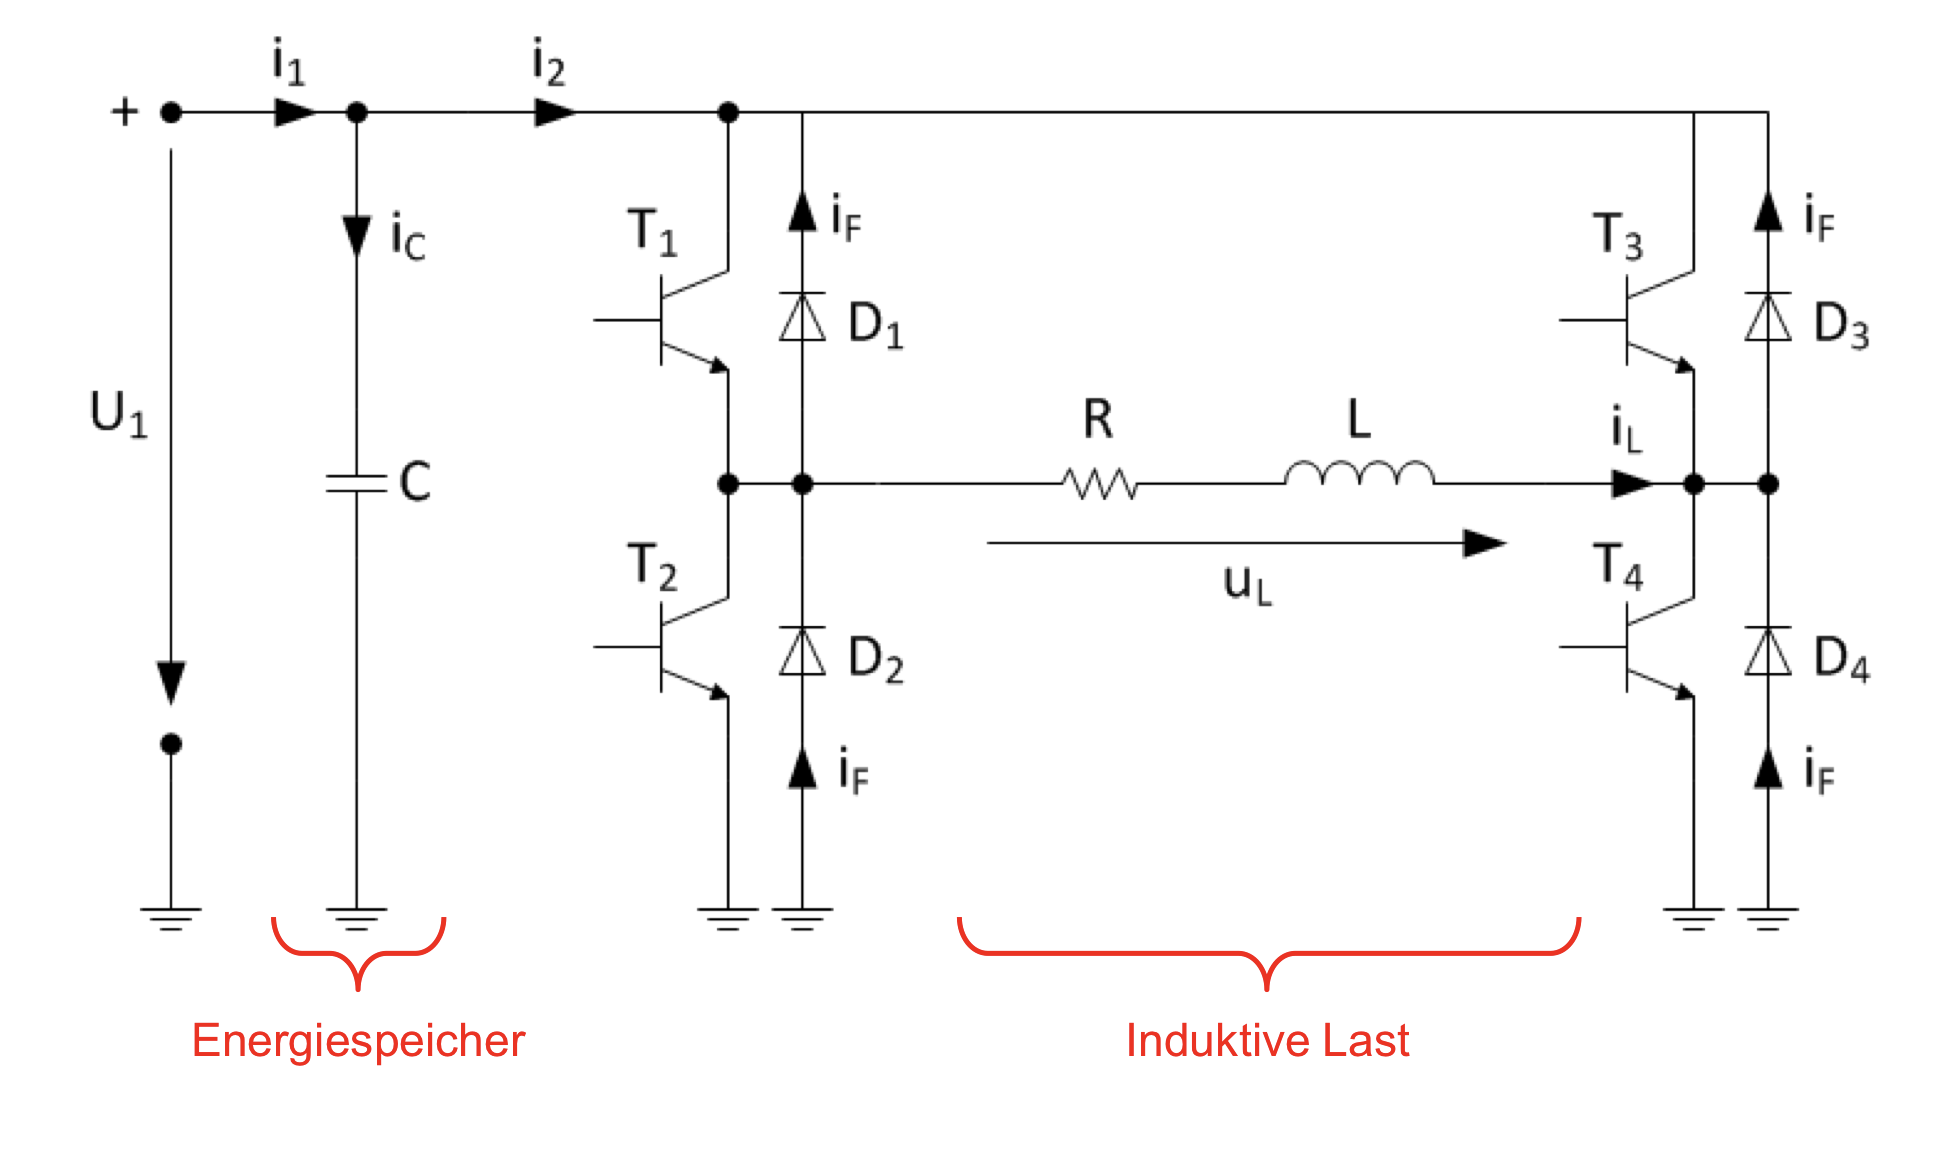
\includegraphics[width=0.85\linewidth]{images/1PWechselrichter.png}
\end{center}

Die H-Brücke besteht aus zwei Halbbrücken:
\begin{itemize}
\item obere Schalter $S_1, S_2$,
\item untere Schalter $S_3, S_4$.
\end{itemize}

Zulässige Schaltzustände:

\begin{center}
\begin{tabular}{c|c|c|c|c}
Zustand & $S_1$ & $S_2$ & $S_3$ & $S_4$ \\ \hline
$+U_{DC}$ & 1 & 0 & 0 & 1 \\
$-U_{DC}$ & 0 & 1 & 1 & 0 \\
Kurzschluss & 1 & 1 & 0 & 0 \\
Kurzschluss & 0 & 0 & 1 & 1 \\
\end{tabular}
\end{center}

\crd{\textrightarrow\ Obere und untere Schalter eines Zweigs dürfen nie gleichzeitig leiten (Shoot-Through).}

\subsection{Rechteckbetrieb (Grundbetrieb)}

Im einfachsten Fall wird die Brücke mit 50\,\% Tastgrad betrieben.

% --- bestehende Grafik: Zeitverlauf ---
\begin{center}
    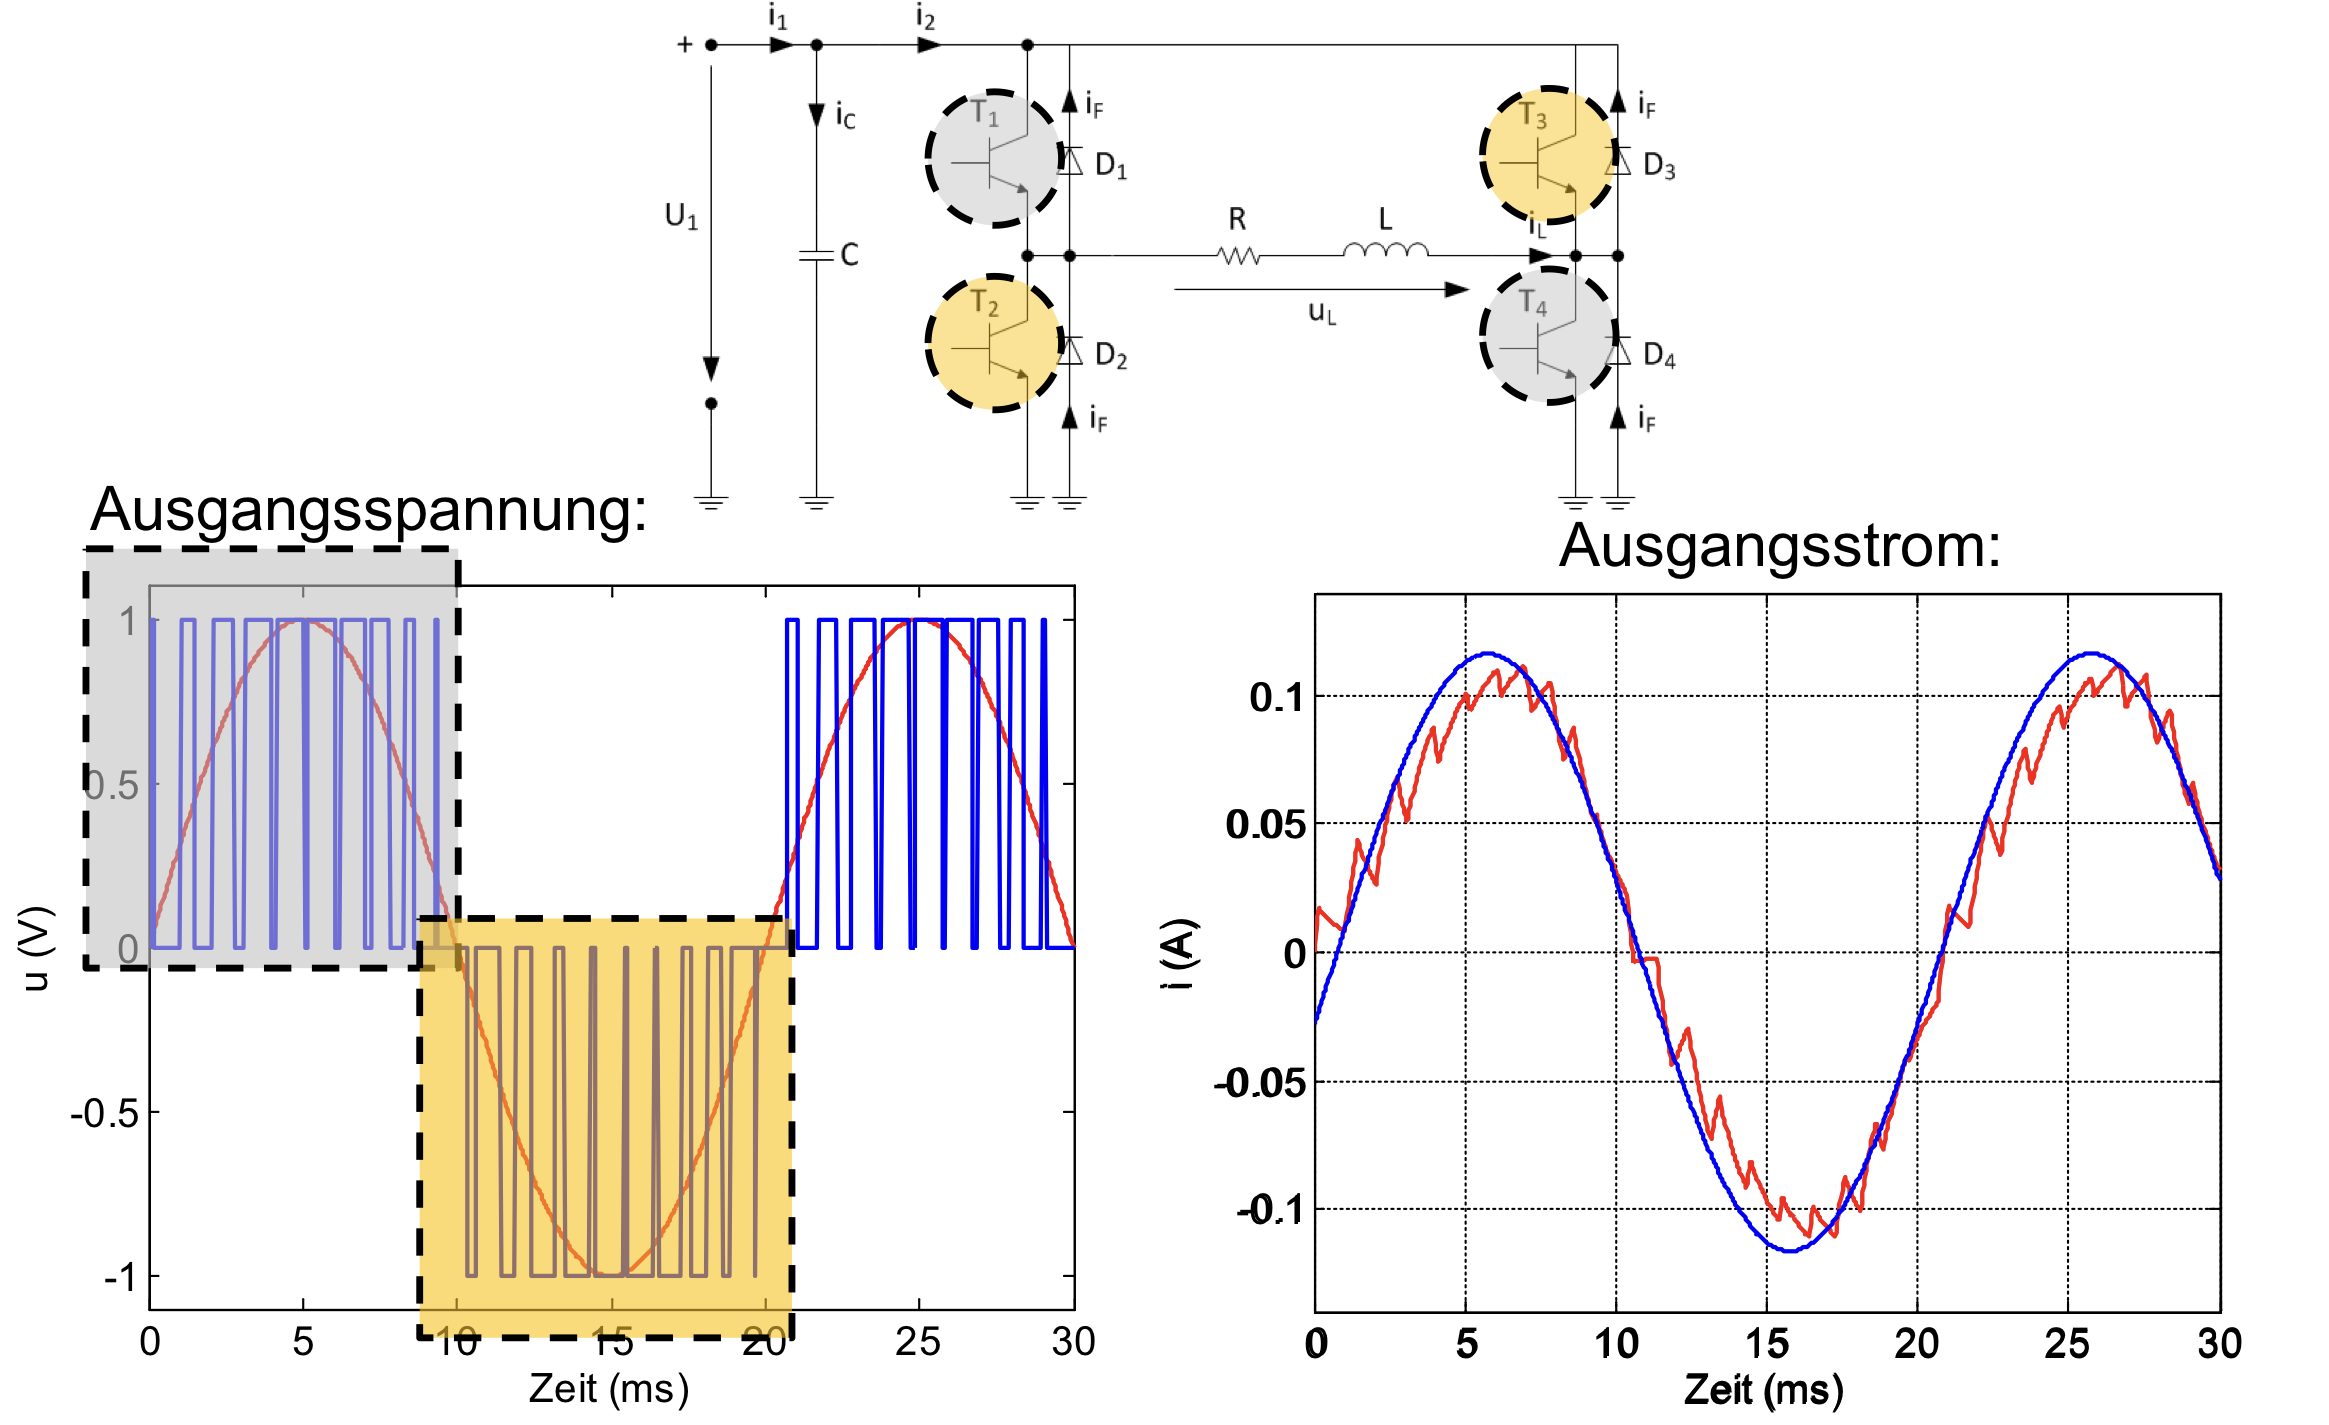
\includegraphics[width=0.85\linewidth]{images/1PWechselrichter_verlauf.png}
\end{center}

Ausgangsspannung:
\[
u_2(t) =
\begin{cases}
+U_{DC}, & 0 < \omega t < \pi \\
- U_{DC}, & \pi < \omega t < 2\pi
\end{cases}
\]

Frequenz:
\[
\boxed{f_2 = \frac{1}{T_2}}
\]

Amplitude:
\[
\boxed{\hat U = U_{DC}}
\]

\subsection{Fourier-Entwicklung des Rechtecksignals}

Fourier-Reihe:

\[
\boxed{
u_2(t) = \frac{4U_{DC}}{\pi} \left[
\sin(\omega t) + \frac{1}{3}\sin(3\omega t) + \frac{1}{5}\sin(5\omega t) + \ldots
\right]
}
\]

Grundschwingung:

\[
\boxed{\hat U_1 = \frac{4}{\pi} U_{DC}}
\]

Effektivwert der Grundschwingung:

\[
\boxed{U_{1,\mathrm{RMS}} = \frac{4}{\pi\sqrt{2}} U_{DC}}
\]

Konsequenzen:
\begin{itemize}
\item Nur ungerade Harmonische vorhanden.
\item Sehr hohe Verzerrung.
\item Keine Amplitudensteuerung möglich.
\end{itemize}

\subsection{Strom bei R--L-Last}

Bei induktiver Last gilt:
\[
i_2(t) = \frac{1}{L} \int u_2(t)\, dt
\]

Eigenschaften:
\begin{itemize}
\item Strom ist \textbf{phasenverschoben} zur Spannung.
\item Strom ist \textbf{glatter} als Spannung (Tiefpasswirkung der Induktivität).
\item Freilaufpfade sind zwingend erforderlich.
\end{itemize}

\subsection{PWM-Betrieb (Sinus-PWM)}

Zur Verbesserung der Spektraleigenschaften wird Pulsweitenmodulation eingesetzt.

Prinzip:
\begin{itemize}
\item Vergleich eines Sinus-Referenzsignals mit einem Dreieck-Trägersignal.
\item Schalter schalten mit hoher Frequenz $f_s$.
\item Grundschwingung folgt dem Sinus.
\end{itemize}

Ausgangsspannung:
\[
u_2(t) = \text{PWM-Signal mit Grundschwingung } u_{2,1}(t)
\]

Grundschwingungsamplitude:

\[
\boxed{\hat U_1 = m_a \frac{U_{DC}}{2}}, 
\qquad 0 \le m_a \le 1
\]

Effektivwert:

\[
\boxed{U_{1,\mathrm{RMS}} = m_a \frac{U_{DC}}{2\sqrt{2}}}
\]

\subsection{Spektrale Eigenschaften}

\subsubsection{Rechteckbetrieb}

\begin{itemize}
\item Nur ungerade Harmonische.
\item Harmonische bei $n = 3,5,7,\ldots$
\item Sehr hohe THD.
\end{itemize}

\subsubsection{PWM-Betrieb}

\begin{itemize}
\item Grundschwingung bei $f_2$.
\item Harmonische um Vielfache von $f_s$.
\item Tieffrequente Harmonische stark reduziert.
\item Filterung durch R--L-Last oder LC-Filter möglich.
\end{itemize}

\subsection{Leistungsfluss}

Momentanleistung:
\[
p(t) = u_2(t)\, i_2(t)
\]

Mittlere Leistung:
\[
\boxed{P = U_{1,\mathrm{RMS}} \, I_{1,\mathrm{RMS}} \cos\varphi_1}
\]

\begin{itemize}
\item Motorbetrieb: $P>0$.
\item Generatorbetrieb: $P<0$ (Rückspeisung möglich bei geeigneter Topologie).
\end{itemize}

\subsection{Typische Betriebsarten}

\begin{itemize}
\item Rechteckbetrieb: einfach, hohe Harmonische.
\item PWM-Betrieb: komplexer, gute Spannungsqualität.
\item Niedrige $f_s$: geringe Schaltverluste, schlechtere Filterbarkeit.
\item Hohe $f_s$: bessere Filterbarkeit, höhere Schaltverluste.
\end{itemize}

\subsection{Vergleich zu Gleichrichtern}

\begin{itemize}
\item Gleichrichter: AC $\rightarrow$ DC.
\item Wechselrichter: DC $\rightarrow$ AC.
\item Beide basieren auf identischer Brückentopologie.
\item Unterschied liegt nur in der Ansteuerung.
\end{itemize}

\subsection{Merksätze}

\begin{itemize}
\item H-Brücke erzeugt $\pm U_{DC}$ am Ausgang.
\item Rechteckbetrieb: keine Amplitudensteuerung, viele Harmonische.
\item PWM: Amplitude über $m_a$ steuerbar.
\item Induktive Last glättet den Strom.
\item Freilaufpfade sind zwingend notwendig.
\item Schaltfrequenz hoch $\Rightarrow$ Filter einfacher, Verluste grösser.
\end{itemize}
